\documentclass{article}
\usepackage{cite}
\usepackage{graphicx}
\usepackage{amsmath}
\usepackage{algorithm}
\usepackage{algpseudocode}

\title{MPU6050 - Sampling Rate and its Effect on the Interrupt Pin}
\author{Roche Christopher \\ \texttt{rochextopher@gmail.com}}

\begin{document}
	\maketitle

	
	\section{Introduction}
	\label{sec:introduction}
	MPU6050 is a sophisticated MEMS that contains 3-axis accelerometer, 3-axis gyroscope and a temperature sensor. It is highly customizable and one of the important aspects of it is the sampling rate which determines the rate at which the sensor data is sampled and made available to the user. 
	
	\section{Background}
	
	\subsection{Pertinent Registers}
	The registers pertinent to this article are discussed in this section. 
	
	\subsubsection{Power Management 1 }
	Address of the power management register is \texttt{0x6B} and the bit representation of the same is given in Figure \ref{fig:pwr_mgmt_reg}.  
	\begin{figure}[h]
		\centering
		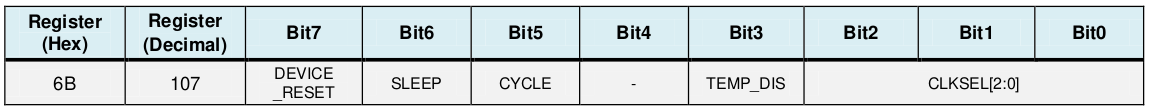
\includegraphics[width=\textwidth]{figs/reg_pwr_mgmt.png}
		\caption{Power Management Register \cite{mpu6050-register-map}}
		\label{fig:pwr_mgmt_reg}
	\end{figure}

	The MPU6050 module is in the state of sleep by default. Reading the power management register would result in the output \textbf{64}, which when converted to binary would be \textbf{01000000}. To wake up the module, 6\textsuperscript{th} bit has to be set to 1.
	
	\begin{figure}[h]
		\centering
		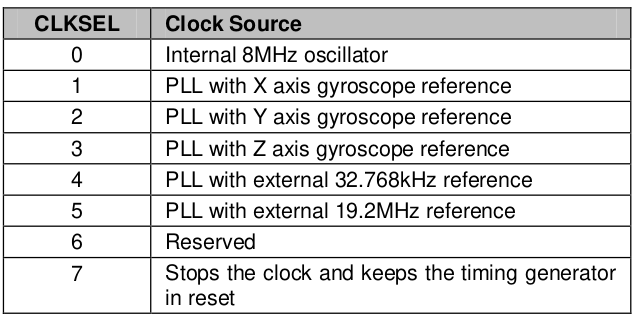
\includegraphics[width=\textwidth]{figs/clk_sel_table.png}
		\caption{Clock Select Table \cite{mpu6050-register-map}}
		\label{fig:clk_sel_table}
	\end{figure}
	
	Additionally, the bits [2:0] can be used to select the clock source of the module. The bits value against the clock source is given in \ref{fig:clk_sel_table}. According to the register map document\cite{mpu6050-register-map}, it is highly
    recommended that the device be configured to use one of the gyroscopes (or an external clock source) as the clock reference for improved stability. 
    
    \subsubsection{Configuration}
    Address of the power management register is \texttt{0x1A} and the bit representation of the same is given in Figure \ref{fig:config_reg}.  
    
    \begin{figure}[h]
    	\centering
    	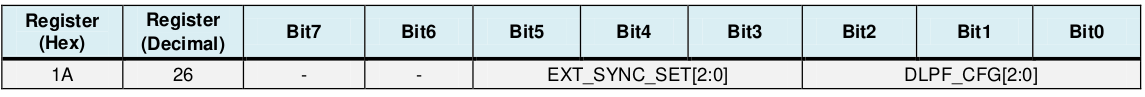
\includegraphics[width=\textwidth]{figs/reg_config.png}
    	\caption{Configuration Register \cite{mpu6050-register-map}}
    	\label{fig:config_reg}
    \end{figure}

	\begin{figure}[h]
		\centering
		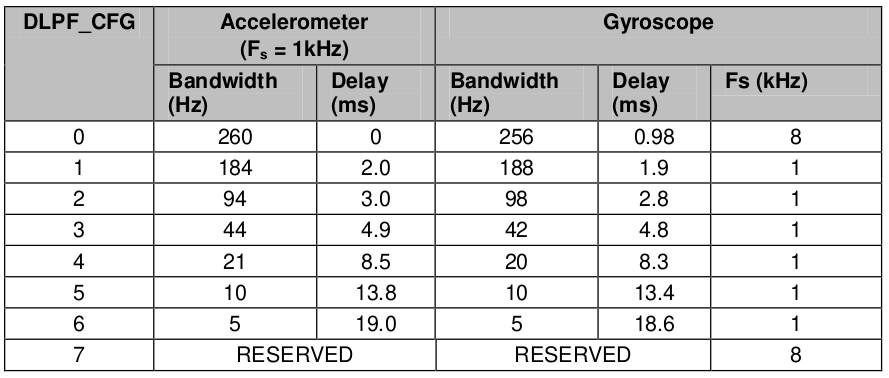
\includegraphics[width=\textwidth]{figs/dlpf_config_table.png}
		\caption{DLPF Configuration Table \cite{mpu6050-register-map}}
		\label{fig:dlpf_config_table}
	\end{figure}

	The noise in the sensor data can be filtered using the in-built Digital Low Pass Filter(DLPF). The bandwidth of the DLPF is determined by the [2:0] bits of the configuration register. The value of the DLPF\_CFG bits and the respective bandwidth is given in the table provided in Figure \ref{fig:dlpf_config_table} along with their delays. Delay represents the latency between the original sensing time and the time at which the data is written to the register.
	

	\subsubsection{Sampling Rate Division}
	\label{sec:smplrt_div}
	Address of the power management register is \texttt{0x19}. The sampling rate, as mentioned in Section \ref{sec:introduction}, is the interval at which the new sensor data is made available to the user. The sensor register output, FIFO output, and DMP sampling are all based on the Sample Rate\cite{mpu6050-register-map}. This can be defined by the user by manipulating the sampling rate division register \textbf{SMPLRT\_DIV}. The sampling rate is calculated as
	
	$$ \text{sampling rate} = \frac{\text{gyroscope output rate}}{1 + \text{smplrt\_div}} $$
	
	So, the value that has to be written to the SMPLRT\_DIV register can be calculated as 
	
	$$ \text{smplrt\_div} = \frac{\text{gyroscope output rate}}{\text{required sampling rate}} \text{ - 1} $$
    
    \subsubsection{Interrupt Enable}
    
    \begin{figure}[h]
    	\centering
    	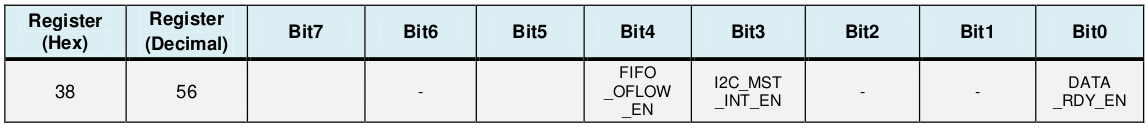
\includegraphics[width=\textwidth]{figs/reg_int_enable.png}
    	\caption{Interrupt Enable Register\cite{mpu6050-register-map}}
    	\label{fig:int_en_reg}
    \end{figure}

    Address of the interrupt enable register is \texttt{0x38}. This register is used to set the interrupt sources. Three different sources can generate interrupt and they are FIFO overflow, I2C master interrupt and data ready. The sources that are set to 1 in this register, as shown in Figure \ref{fig:int_en_reg}, generate an interrupt when a specific action has been done. If \textit{DATA\_RDY\_EN} is set, then an interrupt is generated each time a write operation to all of the sensor registers has been completed\cite{mpu6050-register-map}.
    
    \subsubsection{Interrupt Status}
    \begin{figure}[h]
    	\centering
    	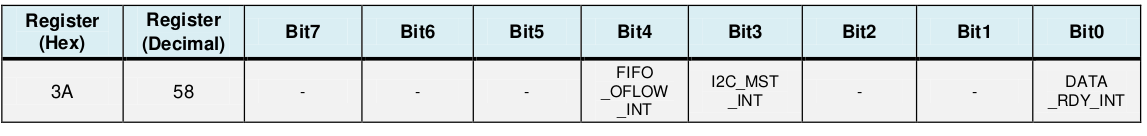
\includegraphics[width=\textwidth]{figs/reg_int_status.png}
    	\caption{Interrupt Status Register\cite{mpu6050-register-map}}
    	\label{fig:int_status_reg}
    \end{figure}
    Address of the interrupt status register is \texttt{0x3A}. This register holds the status of the generated interrupts. This is a \textbf{read only} register. The representation of the bits are shown in Figure \ref{fig:int_status_reg}
    
    \subsubsection{Interrupt Pin Configuration}
    \label{sec:int_pin_cfg}
    \begin{figure}[h]
    	\centering
    	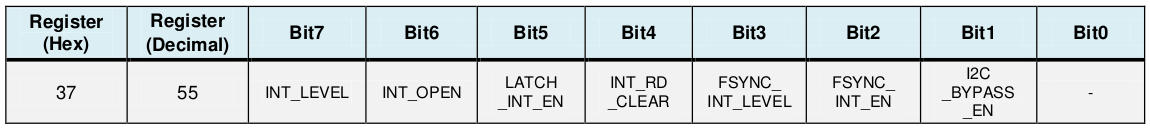
\includegraphics[width=\textwidth]{figs/reg_int_pin_cfg.png}
    	\caption{Interrupt Pin Configuration Register\cite{mpu6050-register-map}}
    	\label{fig:int_pin_cfg}
    \end{figure}
	 Address of the interrupt pin configuration register is \texttt{0x37}. Although registers \texttt{0x38} define the sources that can generate an input, register \texttt{0x37} defines the characteristics and behaviour of the physical interrupt pin.
	 
	 Pertaining to the scope of this article are only bits [7:4] and their effect on the interrupt pin is explained in Table \ref{tab:int_pin_cfg}
	 
	\begin{table}[h]
		\centering
		\begin{tabular}{|c|c|p{8cm}|} % Use p{width} for long text
			\hline
			Bit & Parameter & Behaviour \\ % Header row
			\hline
			7 & INT\_LEVEL & When this bit is equal to 0, the logic level for the INT pin is active high. When this bit is equal to 1, the logic level for the INT pin is active low. \\ 
			\hline
			6 & INT\_OPEN & When this bit is equal to 0, the INT pin is configured as push-pull. When this bit is equal to 1, the INT pin is configured as open drain. \\ 
			\hline
			5 & LATCH\_INT\_EN & When this bit is equal to 0, the INT pin emits a 50µs long pulse. When this bit is equal to 1, the INT pin is held high until the interrupt is cleared. \\ 
			\hline
			4 & INT\_RD\_CLEAR & When this bit is equal to 0, interrupt status bits are cleared only by reading INT\_STATUS (Register 58). When this bit is equal to 1, interrupt status bits are cleared on any read operation. \\ 
			\hline
		\end{tabular}
		\caption{Interrupt Pin Configuration}
		\label{tab:int_pin_cfg}
	\end{table}

	\subsection{Interrupt Pin}
	
	\begin{figure}[H]
		\centering
		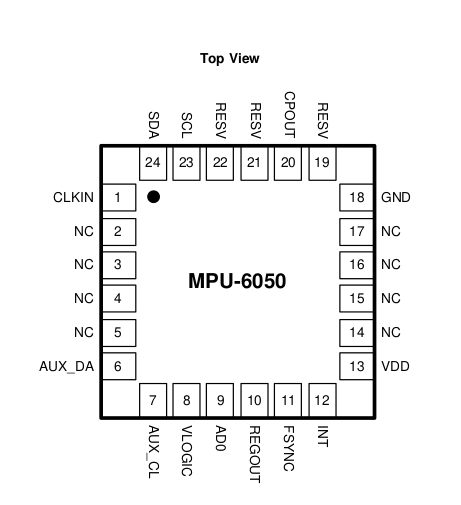
\includegraphics[width=0.8\textwidth]{figs/mpu6050_top_view.png}
		\caption{MPU6050 Top View\cite{mpu6050-product-spec}}
		\label{fig:mpu_top_view}
	\end{figure}

	MPU6050 has an interrupt pin (pin 12) as shown in Figure \ref{fig:mpu_top_view}. This pin is connected to the output of multiple modules internally and it is clearly visible in the block diagram shown in Figure \ref{fig:mpu_block_diagram}. Depending on the register values of 0x3A and 0x37, this pin could be high or low at any moment.
	
	\begin{figure}[H]
		\centering
		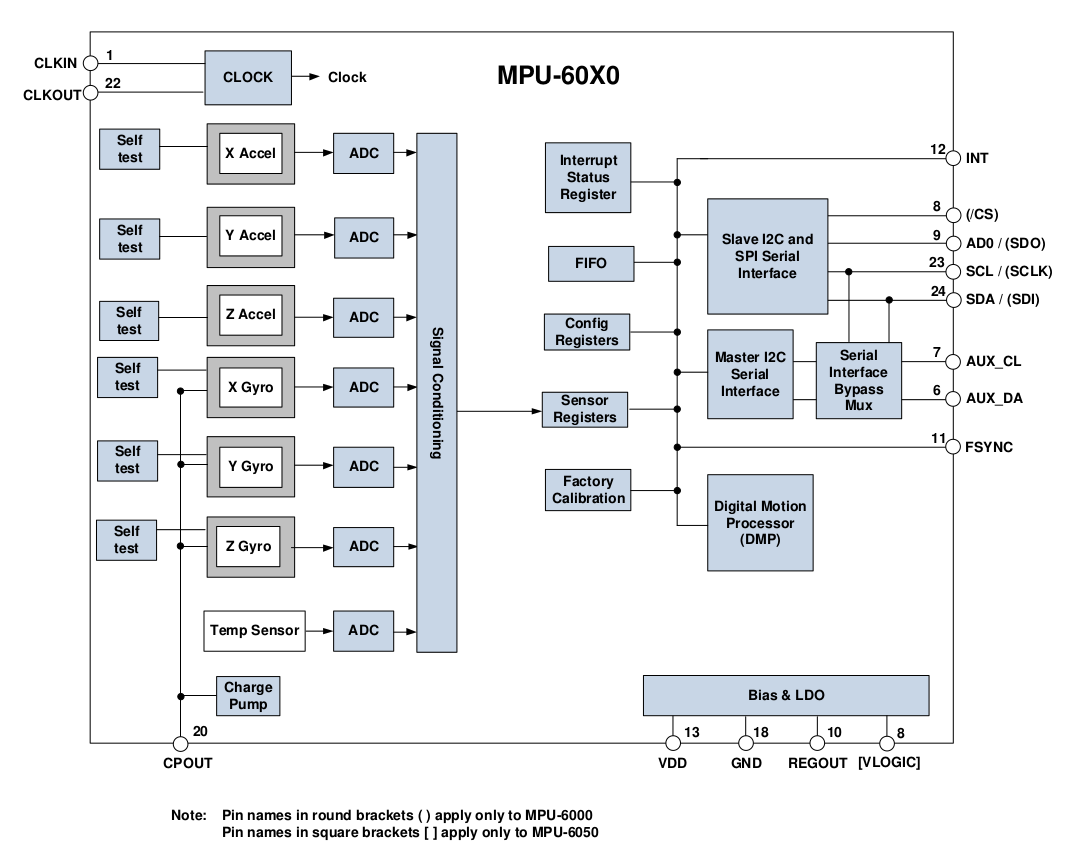
\includegraphics[width=\textwidth]{figs/mpu_block_diagram.png}
		\caption{MPU60X0 Block Diagram\cite{mpu6050-product-spec}}
		\label{fig:mpu_block_diagram}
	\end{figure}

	
	\section{Verification of Sampling Rate Through Interrupt Pin}
	
	\subsection{MPU6050 Setup}
	
	In this setup, we would be using the X axis gyroscope referenced PLL as internal clock source. So the power management register would be set to \texttt{00000001}. 
	
	DLPF could be configured to any bandwidth and to achieve the least latency, it would be configured with 188Hz bandwidth. Hence the config register would be set to \texttt{00000001}. 
	
	We will be monitoring the data ready interrupt and hence that alone should be enabled in order to ignore other events based on I2C and FIFO. So INT\_EN register has to be set with \texttt{00000001}. 
	
	Here comes the complex part, the INT\_PIN\_CFG register. The following characteristics are desired.
	
	\begin{itemize}
		\item Active low
		\item Push-Pull, since no external pull-up would be provided.
		\item Interrupt status remains unless cleared
		\item Interrupt cleared when INT\_EN registered is read
	\end{itemize}
	
	To achieve the abovementioned behaviour, based on Section \ref{sec:int_pin_cfg} and Figure \ref{fig:int_pin_cfg}, the bits to be set are \texttt{10100000}.
	
	The sensor values are made available to the users, as mentioned in Section \ref{sec:smplrt_div}, is determined by the value in register, \texttt{0x19}. For this experiment, we are going to set the sampling rate to 100 Hz. To calculate the value to be put in the register, \texttt{0x19}, the gyroscope output rate should be known. We would be using the DLPF and hence the gyroscope output rate would be 1KHz. So the SMPLRT\_DIV would be 
	
	$$ \text{SMPLRT\_DIV} = \frac{\text{1000}}{\text{100}} \text{ - 1} = 9$$
	So, \texttt{00001001} should be set to the SMPLRT\_DIV register.
	
	
	With the reckoned bit values, a general setup of MPU6050 can be done based on the Algorithm \ref{algo:setup_mpu}.

	
	\begin{algorithm}
		\label{algo:setup_mpu}
		\caption{Setup MPU6050}
		\begin{algorithmic}[1]
			\State Setup power management bits: Wake up
			\State Set configuration bits for DLPF 
			\State Set the sampling rate
			\State Set the interrupt enable bits
			\State Set interrupt pin configuration bits
		\end{algorithmic}
	\end{algorithm}

	\subsection{Verification of Sampling Rate}
	The sampling rate is chosen to be 10 Hz. Depending on our interrupt enable and interrupt pin configuration, the interrupt pin should go low for every 10 ms, provided the interrupt register is read, before the next interrupt. This can be verified easily using a Digital Signal Oscilloscope, but for the lack of it, we are going to use a microcontroller. 
	
	The interrupt pin of the MPU6050 is connected to a GPIO pin that setup to sense the falling edge. A timer is initialized and started after the setup of MPU6050. An Interrupt Service Routine is setup which calculates the interval between each interrupt is setup as shown in Algorithm \ref{algo:isr}. The psuedocode for the verification is provided in Alogrithm \ref{algo:verification}.
	
	 \begin{algorithm}
	 	\label{algo:isr}
	 	\caption{Interrupt Service Routine (ISR)}
	 	\begin{algorithmic}[1]
	 		\State Read the timer count value
	 		\State Read from the MPU6050 Interrupt Status Register
	 		\State Set timer count to 0
	 		\State Print timer count / clock frequency
	 	\end{algorithmic}
	 \end{algorithm}
 
	 \begin{algorithm}
	 	\label{algo:verification}
	 	\caption{Initialize Timer and MPU6050}
	 	\begin{algorithmic}[1]
	 		\State Initialize a timer
	 		\State Setup an interrupt pin
	 		\State Setup the MPU6050: Algo \ref{algo:setup_mpu}
	 		\State Start the timer.
	 	\end{algorithmic}
	 \end{algorithm}
	 

 
	\begin{thebibliography}{9}
		\bibitem{mpu6050-register-map}
		TDK InvenSense,
		\textit{MPU-6050 Register Map}, {https://invensense.tdk.com/wp-content/uploads/2015/02/MPU-6000-Register-Map1.pdf} (Accessed: 9 October 2024).
		
		\bibitem{mpu6050-product-spec}
		TDK InvenSense,
		\textit{MPU-6050 Product Specification}, {https://invensense.tdk.com/wp-content/uploads/2015/02/MPU-6000-Datasheet1.pdf} (Accessed: 9 October 2024).
		
	\end{thebibliography}
\end{document}

